%!TEX root = ../thesis.tex
\chapter{Аналіз застосування GAN для аугментації навчальних вибірок}
\label{chap:practice}

У даному розділі ми застосуємо розглянуті нами у попередніх
частинах моделі та методи на практиці, а саме навчимо варіацію
моделі архітектури UNet з різними функціями помилки. Обрахуємо
метрики і визначимо чи дійсно проблема незбалансованості
класів істотно впливає на якість семантичної сегментації супутникових
знімків. І на сам кінець за допомогою генеративно-змагальних
мереж згенеруємо штучні приклади, які додамо до реальних даних
та будемо проводити навчання вже на ції аугментованій вибірці.
І визначимо чи дійсно подібний спосіб дозволяє
покращити якість семантичної сегментації.

Вихідний код, який був створено для усіх наведених у даному
розділі експериментів доступний на GitHub
\footnote{\href{https://github.com/ShkalikovOleh/SatelliteGAN}
    {https://github.com/ShkalikovOleh/SatelliteGAN}}.

\section{Попередня обробка навчальних даних}

Для перевірки того, чи дійсно запропонований підхід
дозволить збільшити якість семантичної сегментації супутникових знімків
проведемо експерименти з класифікації на 19 класів
композиту Sentinel-2A \cite{drusch2012sentinel}
для Київської області взятих з 1 липня по 1 серпня 2021 року.
Класи представляють собою здебільшого сільськогосподарські
культури, тому розв'язання задачі сегментації саме на таких
даних має широкий прикладний потенціал.

Ми використовували саме композит супутникових знімків, бо
територія Київської області надто велика, щоб вона могла
повністю розміститися на одному супутниковому знімку Sentinel-2A.
Саме тому був взятий часовий ряд червоного, зеленого, синього та
ближнього інфрачервоного каналів за липень 2021~р., який потім був об'єднаний.
У тих частинах, що перетиналися були, були обрані медіанні значення
пікселів, також знімки були очищені від детектованих хмар та тіней від них.

Після чого ці дана колекція знімків була об'єднана у один
великий композит для Київської області та до цього композиту
була додана окремим каналом маска з мітками класів, яка була
отримана у результаті досліджень науковцями інституту
космічних досліджень Національної академії наук України.

Сучасні нейромережеві архітектури не дозволяють нам працювати
з зображення дуже великого розміру, тому ми вимушені
розрізати отриманий композит на квадратні частини розміром $256 \times 256$
пікселів. Такий вибір обґрунтований тим, що саме такий розмір
зображення генерувався авторами класичного Pix2Pix  \cite{pix2pix}.

Попри те, що ми брали дані за місяць, все одно залишились
території, які не були покриті супутником за спостережуваний період.
До того ж, контури Київської області не є ідеальною геометричною фігурою,
тож на деяких знімках, на яких показані кордони області відсутні значення
пікселів або масок, які відповідають іншим областям.
Через ці два фактори у деяких отриманих зображеннях
присутні пікселі, у яких відсутнє значення.
Такі приклади були відфільтровані та не
використовувалися при навчанні нейронних мереж.

На сам кінець, через те, що використовувалися знімки з
попередньою обробкою та корекцією класу TOA, то
область значень кожного з каналів була не класичною
$[0, 1]$, а мала більше максимальне значення.
У свою чергу більшість нейромережевих архітектур працює зі
значеннями у проміжку $[-1, 1]$.
Тож був застосований аналог min-max нормалізації, а саме
кожне значення пікселю кожного каналу було поділено на
максимальне значення для даного каналу даного зображення,
а після цього класична стандартизація з математичним
сподівання і стандартним відхиленням рівними $0.5$.

\section{Результати сегментації без використання GAN}

Для розв'язання задачі семантичної сегментації
даної вибірки супутникових знімків було використано
архітектуру UNet. Для того, щоб ми мали змогу перевірити
якість моделі використовуючи метрики, і при цьому
отримали достовірні значення, тобто уникнули явища
перенавчання, вибірку було поділено навпіл на навчальну і тестову.

У якості енкодера у використаній варіації UNet було обрано
ResNet-34, що є компромісом між обчислювальною потужністю,
необхідною для навчання подібних моделей та
складністю мережі.

Дана вибірка є незбалансованою, що можна побачити на
статистиках по сумарній кількості пікселів
для кожного класів на рисунку \ref{fig:pixels_per_class}
(мітки класів відповідають назвам, які можна знайти
у таблиці \ref{tab:segm_result_real_per_classes}).
Тож для подолання проблем, які пов'язані з цим, ми спробували
застосувати різні функції помилок, а саме зважені та
не зважені Cross-Entropy
та Focal Loss. У якості вагових коефіцієнтів для кожного
класу були обрані нормовані зворотні відношення сумарної кількості пікселів класу
до кількості усіх пікселів у тренувальній вибірці.

У якості оптимізатора було обрано добре відомий,
один з найбільш застосовуваних та ефективних,
алгоритм Adam \cite{kingma2014adam} зі швидкістю навчання
$2 \cdot 10^{-4}$. Розмір батчу дорівнював $64$.

\begin{table}[!ht]
    \centering
    \caption{Глобальні метрики точності сегментації
        для реальної вибірки}
    \begin{tabular}{|c|C|C|C|C|}
        \hline
        \multirow{2}{*}{Метрика} & \multicolumn{2}{c|}{CE Loss} & \multicolumn{2}{c|}{Focal Loss}                                   \\
        \cline{2-5}              & w/o W                        & W                               & w/o W          & W              \\
        \hline $\acc$            & 0.76                         & 0.738                           & \textbf{0.762} & 0.755          \\
        \hline $\varkappa$       & 0.72                         & 0.697                           & \textbf{0.722} & 0.716          \\
        \hline $\iou$            & 0.356                        & 0.352                           & 0.363          & \textbf{0.368} \\
        \hline
    \end{tabular}
    \label{tab:segm_result_real_global}
\end{table}

У результаті $500$-та епох навчання було отримані значення
метрик, таких як точність ($\acc$), міра Жаккара ($\iou$) та
каппа Коена ($\varkappa$), для різних варіацій функції помилки.
Вони наведені у таблиці \ref{tab:segm_result_real_global}
(w/o W означає не зважену помилку, W -- зважену).

Що стосується якості сегментації за кожним з класів, то
слід звернутися до таких метрик як Producer Accuracy $\pracc$
та User Accuracy $\usacc$, наведених у таблиці \ref{tab:segm_result_real_per_classes}.

\begin{table}[!ht]
    \centering
    \caption{Метрики точності сегментації за класами
        для реальної вибірки}
    \begin{tabular}{|K|C|C|C|C|C|C|C|C|}
        \hline
        \multirow{3}{*}{Назва класу}   & \multicolumn{4}{c|}{PA}         & \multicolumn{4}{c|}{UA}                                                                                                               \\
        \cline{2-9}
                                       & \multicolumn{2}{c|}{CE Loss}    & \multicolumn{2}{c|}{Focal Loss} &
        \multicolumn{2}{c|}{CE Loss}   & \multicolumn{2}{c|}{Focal Loss}                                                                                                                                         \\
        \cline{2-9}
                                       & w/o W                           & W                               & w/o W          & W              & w/o W          & W              & w/o W          & W              \\
        \hline Штучні об'єкти          & 0.64                            & \textbf{0.66}                   & 0.649          & 0.652          & 0.664          & 0.59           & \textbf{0.68}  & 0.668          \\
        \hline Зернові культури        & 0.822                           & 0.772                           & \textbf{0.825} & 0.791          & 0.718          & 0.712          & 0.721          & 0.734          \\
        \hline Ріпак                   & 0.285                           & 0.285                           & 0.272          & \textbf{0.297} & \textbf{0.533} & 0.404          & 0.533          & 0.458          \\
        \hline Гречка                  & 0.012                           & 0.038                           & 0.032          & \textbf{0.047} & 0.151          & 0.059          & \textbf{0.165} & 0.1            \\
        \hline Кукурудза               & 0.882                           & 0.825                           & \textbf{0.887} & 0.861          & 0.837          & \textbf{0.853} & 0.834          & 0.85           \\
        \hline Буряк                   & 0.27                            & 0.356                           & 0.324          & \textbf{0.367} & 0.472          & 0.417          & \textbf{0.537} & 0.435          \\
        \hline Соняшник                & \textbf{0.887}                  & 0.848                           & 0.881          & 0.866          & 0.83           & 0.83           & 0.839          & \textbf{0.844} \\
        \hline Соя                     & 0.581                           & \textbf{0.64}                   & 0.595          & 0.608          & 0.715          & 0.584          & \textbf{0.716} & 0.662          \\
        \hline Інші культури           & 0.09                            & \textbf{0.207}                  & 0.09           & 0.201          & 0.222          & 0.162          & \textbf{0.233} & 0.192          \\
        \hline Ліс                     & 0.915                           & 0.827                           & \textbf{0.918} & 0.897          & 0.894          & \textbf{0.931} & 0.897          & 0.913          \\
        \hline Необроблювані землі     & 0.726                           & 0.592                           & \textbf{0.741} & 0.686          & 0.683          & \textbf{0.723} & 0.692          & 0.716          \\
        \hline Відкритий ґрунт         & 0.464                           & 0.694                           & 0.494          & \textbf{0.696} & \textbf{0.573} & 0.392          & 0.57           & 0.438          \\
        \hline Вода                    & \textbf{0.967}                  & 0.964                           & 0.962          & 0.959          & 0.939          & 0.927          & \textbf{0.94}  & \textbf{0.94}  \\
        \hline Болото                  & 0.315                           & \textbf{0.5}                    & 0.308          & 0.434          & 0.461          & 0.287          & \textbf{0.476} & 0.369          \\
        \hline Ячмінь                  & 0.205                           & \textbf{0.292}                  & 0.206          & 0.28           & 0.309          & 0.265          & \textbf{0.317} & 0.3            \\
        \hline Горох                   & 0.01                            & \textbf{0.018}                  & 0.014          & 0.016          & 0.101          & 0.03           & \textbf{0.135} & 0.075          \\
        \hline Трави                   & 0.011                           & \textbf{0.051}                  & 0.016          & 0.038          & 0.083          & 0.05           & 0.1            & \textbf{0.111} \\
        \hline Сади, парки, лісополоси & 0.51                            & 0.496                           & \textbf{0.522} & 0.495          & 0.491          & 0.433          & \textbf{0.498} & 0.486          \\
        \hline Виноградники            & 0.039                           & 0.344                           & 0.01           & \textbf{0.345} & 0.169          & 0.09           & \textbf{0.197} & 0.144          \\
        \hline
    \end{tabular}
    \label{tab:segm_result_real_per_classes}
\end{table}

Як можна побачити, за усіма метриками, які є глобальними
перевагу має нейромережа архітектури UNet, яка
при навчанні використовувала не зважену функцію
помилки FocalLoss, а саме вона переважає у Accuracy та
каппі Коена, у той же час відставання за метрикою $\iou$
від лідера не значне.

Що стосується результатів метрик за
кожним окремим класом, то тут бачимо той факт, що як і
очікувалось ті класі, які є міноритарними, тобто кількість їх
пікселів мала відносно інших класів, мають значно нижчі показника,
аніж мажоритарні. Але і для цих метрик мережа, що
навчалась з не зваженим Focal Loss видає переважно кращі
результати, особливо, якщо звернути увагу
на User Accuracy, де така варіацію UNet переважає
для 11 класів, більшість з яких саме міноритарні.
Значення метрики Producer Accuracy теж є достатньо
високими: за 5 класами підхід з використання цієї функції
помилки є найкращими (у той час як лідер переважає у
7 класах), а для інших теж показує гарні результати.

\section{Результати сегментації з використанням аугментованого набору даних}

Як ми переконались, незбалансованість класів дуже
істотно впливає на якість семантичної сегментації супутникових
знімків. Тож спробуємо доповнити нашу вибірку, таким чином збалансувавши її.
Для цього використаємо розроблений нами процес аугментації
за допомогою генеративно-змагальних мереж.

\subsection{Генерація доповнених вибірок}

Перш за все були навчені GAN архітектури Pix2Pix та її варіацію
(будемо позначати її Pix2Pix + HD),
що використовує ті покращення, що
описані у розділі \ref{chap:gans}, а саме:
декілька дискримінаторів та функції помилки узгодженості
ознак~\eqref{eq:fm_loss} та узгодженості внутрішніх представлень
навченої мережі класифікації~\eqref{eq:perceptual_loss}.

Навчання відбувалося протягом 500 епох з використання
оптимізатора Adam \cite{kingma2014adam} зі швидкістю навчання
$2 \cdot 10^{-4}$. У якості параметрів експоненційного
середнього ($\beta_1, \beta_2$) використовувались
значення $0.5, 0.999$ відповідно. Розмір батчу був невеликий і
дорівнював $8$, бо великі значення можуть приводити до
зниження якості згенерованих зображень.

Приклади справжніх зображень (лише червоний, зелений та синій канал)
та тих, які генерують навченні
генеративно-змагальні мережі наведені на рисунках
\ref{fig:real_examples} -- \ref{fig:gen_pix2pix_hd_examples}.

\begin{figure}[ht]
    \centering
    \begin{subfigure}[b]{0.3\textwidth}
        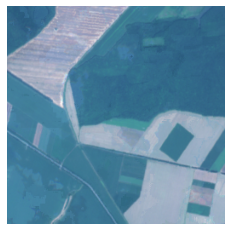
\includegraphics[scale=0.5]{real_0.png}
    \end{subfigure}
    \begin{subfigure}[b]{0.3\textwidth}
        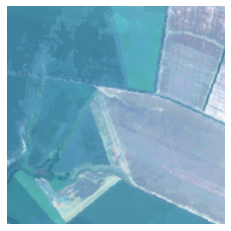
\includegraphics[scale=0.5]{real_1.png}
    \end{subfigure}
    \begin{subfigure}[b]{0.3\textwidth}
        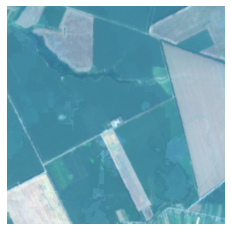
\includegraphics[scale=0.5]{real_2.png}
    \end{subfigure}
    \caption{Приклади справжніх супутникових знімків}
    \label{fig:real_examples}
\end{figure}

\begin{figure}[ht]
    \centering
    \begin{subfigure}[b]{0.3\textwidth}
        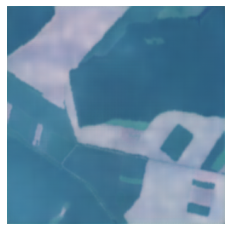
\includegraphics[scale=0.5]{gen_pix2pix_0.png}
    \end{subfigure}
    \begin{subfigure}[b]{0.3\textwidth}
        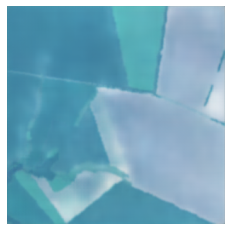
\includegraphics[scale=0.5]{gen_pix2pix_1.png}
    \end{subfigure}
    \begin{subfigure}[b]{0.3\textwidth}
        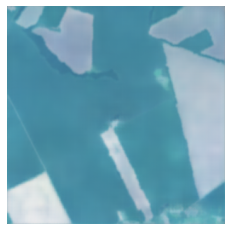
\includegraphics[scale=0.5]{gen_pix2pix_2.png}
    \end{subfigure}
    \caption{Приклади згенерованих Pix2Pix зображень}
    \label{fig:gen_pix2pix_examples}
\end{figure}

\begin{figure}[ht]
    \centering
    \begin{subfigure}[b]{0.3\textwidth}
        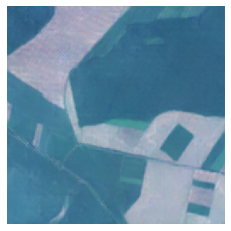
\includegraphics[scale=0.5]{gen_pix2pix_hd_0.png}
    \end{subfigure}
    \begin{subfigure}[b]{0.3\textwidth}
        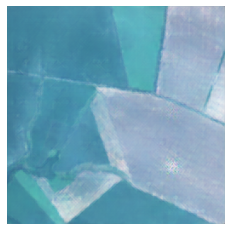
\includegraphics[scale=0.5]{gen_pix2pix_hd_1.png}
    \end{subfigure}
    \begin{subfigure}[b]{0.3\textwidth}
        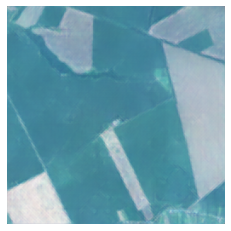
\includegraphics[scale=0.5]{gen_pix2pix_hd_2.png}
    \end{subfigure}
    \caption{Приклади згенерованих Pix2Pix + HD зображень}
    \label{fig:gen_pix2pix_hd_examples}
\end{figure}

Як ми бачимо, на згенерованих прикладах присутня
деяка розмитість та інші незначні артефакти, проти
вони виглядають наближеними до справжніх. Причому візуально
знімки згенеровані модифікацією Pix2Pix виглядають краще.
До того ж,
як ми вже зазначали, кінцевою нашою метою є саме покращення
якості сегментації, а не генерація ідеальних зображень.


Наступним етапом було застосування алгоритму \ref{alg:mask_gen} генерації
штучних масок. Як можна побачити на рисунку \ref{fig:real_examples}
у досліджуваному наборі даних дуже сильний дисбаланс у кількості
пікселів для кожного з класів, тому якщо ми будемо намагатися
зробити повністю рівномірний розподіл, то нам потрібно буде
згенерувати дуже багато штучних зображень, що
може тільки зменшити метрики якості семантичної сегментації.
Тож було обрано наступний підхід: за цільові значення кількості пікселів
обрано $70\%$ від кількості пікселів класу <<Зернові культури>>.
У якості параметру $l$ алгоритму було обрано $2$. При чому
у прикладних застосуваннях нас цікавить підвищення якості класифікації не усіх
класів, а лише окремих, як наприклад нас не цікавить розпізнавання
штучних об'єктів, у тому числі будинків та автомобілів,
якщо ми вирішуємо задачі, які пов'язані з сільськогосподарськими
культурами. Тож ми використали властивість розробленого алгоритму,
яка полягає у тому, що він дозволяє обирати
класи, які будуть доповнюватись, та доповнили наступні класи:
ріпак, гречка, буряк, соя, інші культури, виноградники, трави,
горох, ячмінь.

Усього було згенеровано $1252$ нових приклади кожної з навчених
генеративно-змагальних мереж, і усі вони були додані до
вихідної тренувальної вибірки, таким чином ми отримали аугментовану вибірку.
Статистика по кількості пікселів у доповненій вибірці наведена на
рисунку \ref{fig:pixels_per_class_aug}. Як можна побачити,
класи, які нас особливо цікавлять, стали набагато більш збалансовані.

\begin{figure}[ht!]
    \centering
    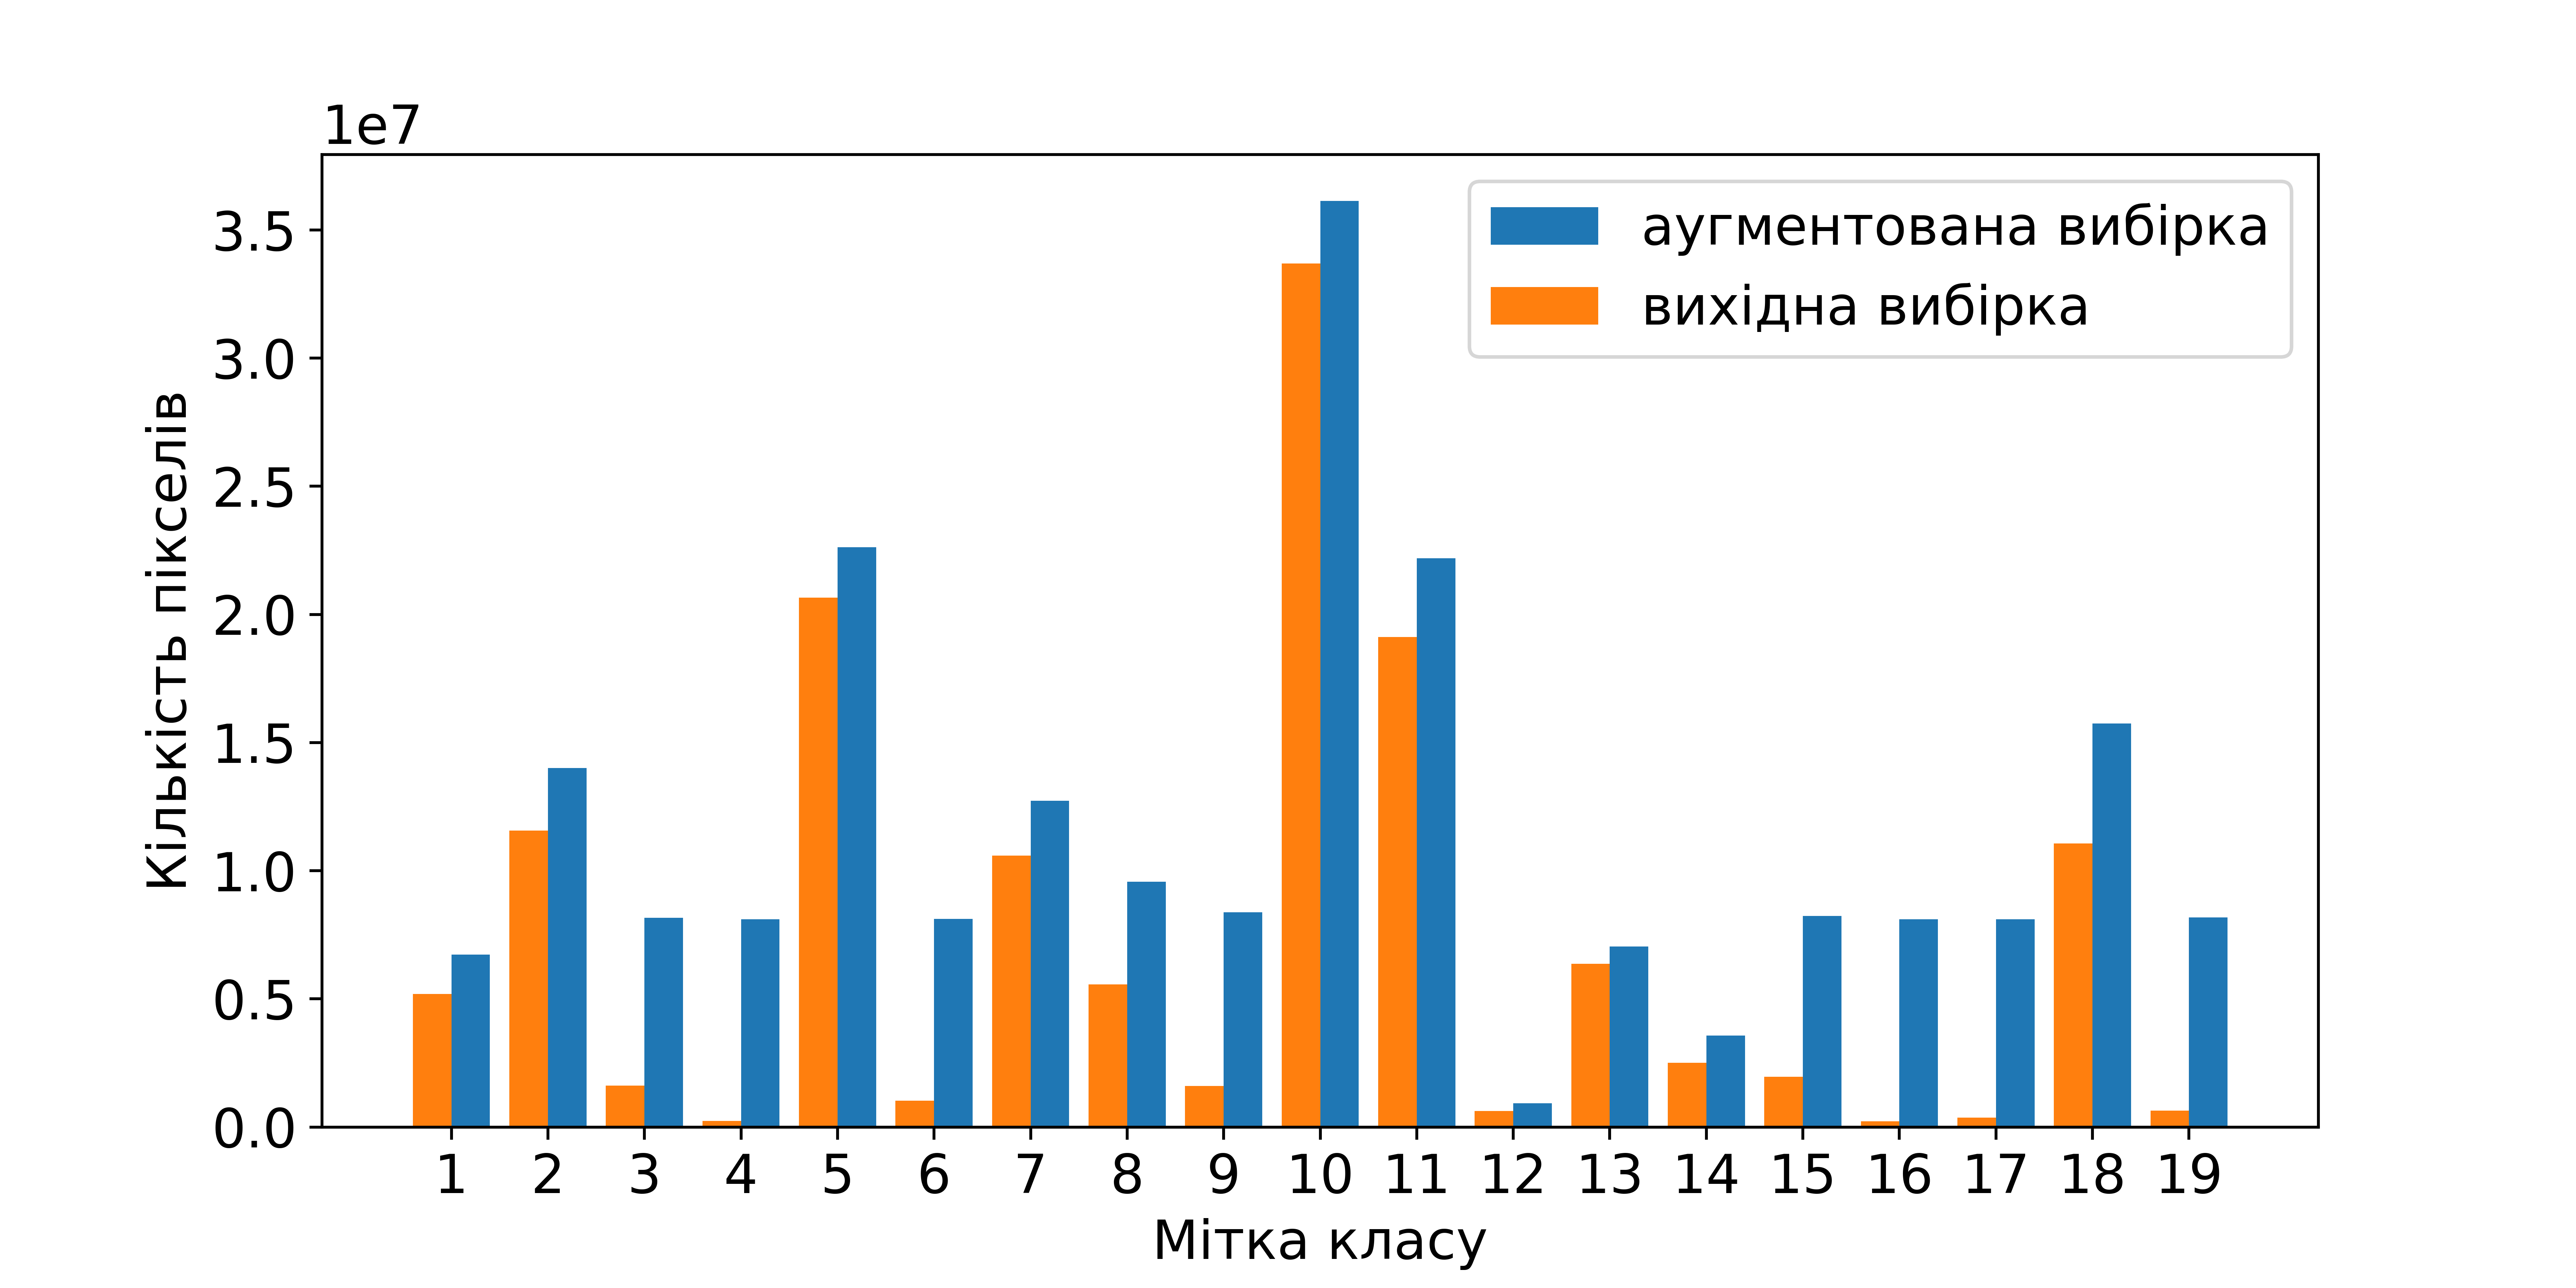
\includegraphics[scale=0.65]{dist_aug_real.png}
    \caption{Порівняння кількості пікселів для різних класів
        у досліджуваному та аугментованому наборах даних}
    \label{fig:pixels_per_class_aug}
\end{figure}

\subsection{Аналіз якості семантичної сегментації при застосуванні
    доповнених вибірок}

Маючи аугментовану вибірку ми маємо змогу перейти до перевірки
нашої гіпотези про те, що генеративно-змагальні мережі
здатні допомогти підвищити якість семантичної сегментації. Для цього,
щоб порівнювати з результатами на вихідній навчальній вибірці,
ми теж навчаємо мережу архітектури UNet з енкодером ResNet-34.
Усі параметри навчання були обрані таки ми же, окрім кількості
епох, яка була зменшена до $300$ через те, що ми працюємо з
більшою вибіркою.

Результати у вигляді метрики точності по класам наведені у
таблиці~\ref{tab:segm_result_augm_per_classes}.

\newcolumntype{S}{>{\centering\arraybackslash}m{1.3cm}}
\newcolumntype{M}{>{\centering\arraybackslash}p{2.2cm}}

\begin{table}[!ht]
    \centering
    \caption{Порівняння метрик
        точності сегментації за кожним класом
        для доповненої вибірки та вихідної вибірок}
    \begin{tabular}{|K|S|C|C|S|C|C|}
        \hline
        \multirow{3}{*}{Назва класу}         & \multicolumn{3}{c|}{PA}                   & \multicolumn{3}{c|}{UA}                                                              \\
        \cline{2-7}
                                             & \multirow{2}{1.3cm}{Вихідна вибірка}      & \multicolumn{2}{M|}{Аугментована вибірка} &
        \multirow{2}{1.3cm}{Вихідна вибірка} & \multicolumn{2}{M|}{Аугментована вибірка}                                                                                        \\
        \cline{3-4} \cline{6-7}
                                             &                                           & Pix2Pix                                   & Pix2Pix + HD &  & Pix2Pix & Pix2Pix + HD \\
        \hline Штучні об'єкти                & 0.649                                     &                                           &              &  &         &              \\
        \hline Зернові культури              & 0.825                                     &                                           &              &  &         &              \\
        \hline Ріпак                         & 0.272                                     &                                           &              &  &         &              \\
        \hline Гречка                        & 0.032                                     &                                           &              &  &         &              \\
        \hline Кукурудза                     & 0.887                                     &                                           &              &  &         &              \\
        \hline Буряк                         & 0.324                                     &                                           &              &  &         &              \\
        \hline Соняшник                      & 0.881                                     &                                           &              &  &         &              \\
        \hline Соя                           & 0.595                                     &                                           &              &  &         &              \\
        \hline Інші культури                 & 0.09                                      &                                           &              &  &         &              \\
        \hline Ліс                           & 0.918                                     &                                           &              &  &         &              \\
        \hline Необроблювані землі           & 0.741                                     &                                           &              &  &         &              \\
        \hline Відкритий ґрунт               & 0.494                                     &                                           &              &  &         &              \\
        \hline Вода                          & 0.962                                     &                                           &              &  &         &              \\
        \hline Болото                        & 0.308                                     &                                           &              &  &         &              \\
        \hline Ячмінь                        & 0.206                                     &                                           &              &  &         &              \\
        \hline Горох                         & 0.014                                     &                                           &              &  &         &              \\
        \hline Трави                         & 0.016                                     &                                           &              &  &         &              \\
        \hline Сади, парки, лісополоси       & 0.522                                     &                                           &              &  &         &              \\
        \hline Виноградники                  & 0.01                                      &                                           &              &  &         &              \\
        \hline
    \end{tabular}
    \label{tab:segm_result_augm_per_classes}
\end{table}

Найкращі показники має

Якщо ж казати про  глобальні метрик , то вони наведені у таблиці
\ref{tab:segm_result_aug_global}.

\begin{table}[!ht]
    \centering
    \caption{Порівняння глобальних метрик
        точності сегментації
        для доповненої вибірки та вихідної вибірок}
    \begin{tabular}{|c|S|C|C|}
        \hline
        \multirow{2}{*}{Метрика} & \multirow{2}{1.3cm}{Вихідна вибірка} & \multicolumn{2}{M|}{Аугментована вибірка}                \\
        \cline{3-4}              &                                      & Pix2Pix                                   & Pix2Pix + HD \\
        \hline $\acc$            & 0.762                                &                                           &              \\
        \hline $\varkappa$       & 0.722                                &                                           &              \\
        \hline $\iou$            & 0.363                                &                                           &              \\
        \hline
    \end{tabular}
    \label{tab:segm_result_aug_global}
\end{table}



Отримані результати свідчать про те, що

\chapconclude{\ref{chap:practice}}

У даному розділі було проведено велику кількість експериментів
з застосуванням супутникових даних Sentinel-2 для Київської області,
взятих за період з 1 липня по 1 серпня 2021 року. Було детальну
описано методи отримання та попередньої обробки даних, які
після цього були поділені на тренувальну та тестову вибірки, які
використовувалися у подальшому.

Було проаналізовано вплив різних функцій помилки, а саме
крос-ентропії та Focal Loss з використанням та без використання вагів.
Було обраховані як глобальні метрики якості семантичної сегментації, так
і для кожного з класів. У результаті було визначено, що
найкращі показники має не зважений Focal Loss.

Генеративно-змагальні мережі архітектури Pix2Pix та її варіацію, що
використовує дискримінатор та функції помилки із архітектури Pix2PixHD
були навчені на даному наборі даних. Якість згенерованих зображень
модифікації виявилась більшою за стандартний Pix2Pix.

Врешті решт було застосовано, описаний у попередніх розділах,
процес доповнення навчальної вибірки для тих класів, які
мали особливе значення. Результати якості по класам дозволять стверджувати,
що запропонований підхід дозволив значно підвищити якість
міноритарних класів. При цьому деякі метрики для глобальних класів незначно
погіршились. Якщо ж порівнювати різні GAN, то тут як і у випадку з
якістю згенерованих зображень перевагу має модифікація Pix2Pix + HD.
Глобальні метрики теж свідчать про те, що загальна якість
семантичної сегментації при застосуванні аугментованих вибірок
не погіршилась.
